% ARSPI-Net measurement-substrate overview (TAFFC variant only).
% Composite "graphical overview" placed early in the manuscript so a reader
% grasps the pipeline by page 2-3: affective ERP observation -> fixed LIF
% reservoir / BSC6 transformation -> four operationally distinct evidence
% streams (E, D, T, C) -> mechanism ablation / perturbation robustness /
% closed-loop evidence accumulation.
%
% Authenticity: the two data anchors are the real, de-identified published
% panels obs01 (grand-average ERP) and obs04 (reservoir spike raster). No
% data is reconstructed or altered; the stream/analysis stages are schematic.
%
% Build (from figures/taffc/):
%   pdflatex fig_arspi_overview.tex
\documentclass[border=3pt]{standalone}
\usepackage{graphicx}
\usepackage{amsmath}
\usepackage{helvet}
\renewcommand{\familydefault}{\sfdefault}
\usepackage{tikz}
\usetikzlibrary{positioning,arrows.meta,fit,backgrounds}
\graphicspath{{../tcds_ready9/observations/}{../../figures/tcds_ready9/observations/}}

\begin{document}
\hyphenpenalty=10000\exhyphenpenalty=10000
\begin{tikzpicture}[
  font=\footnotesize,
  >={Stealth[length=2.4mm]},
  panel/.style={draw, rounded corners, inner sep=2pt},
  title/.style={font=\small\bfseries, align=center},
  sub/.style={font=\scriptsize, align=center, text=black!70},
  stream/.style={draw, rounded corners, fill=black!4, align=flush left,
                 text width=3.15cm, inner sep=3pt, minimum height=0.60cm},
  analysis/.style={draw, rounded corners, fill=black!7, align=flush left,
                   text width=3.5cm, inner sep=3pt, minimum height=0.82cm},
  flow/.style={->, very thick, black!60},
]

% ---- Stage 1: affective ERP observation (real panel obs01) ----
\node[panel] (erp) {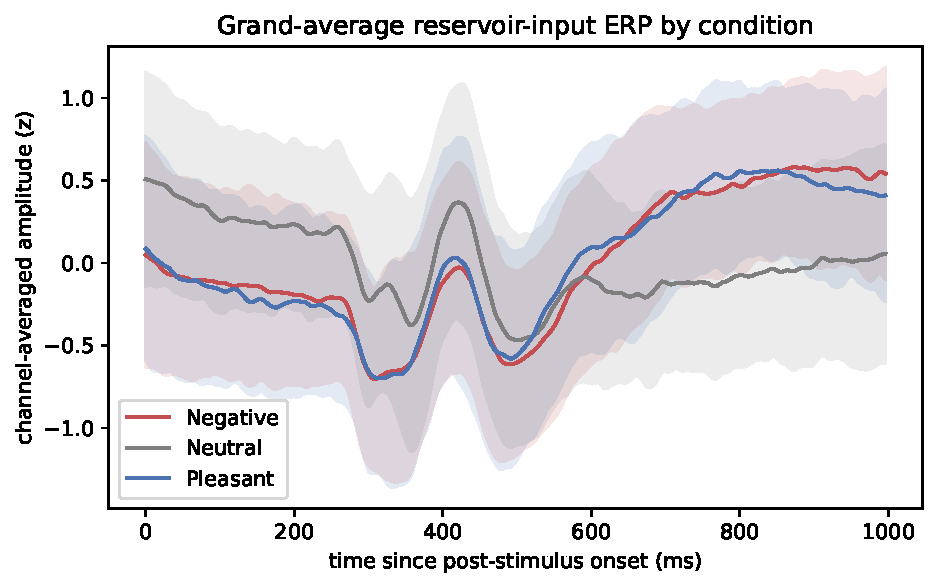
\includegraphics[width=3.5cm]{obs01_erp_condition_grand_average}};
\node[title, above=1.5pt of erp] {Affective ERP observation};
\node[sub, below=1.5pt of erp, text width=3.7cm] {trial-averaged response per condition\\(negative / neutral / pleasant)};

% ---- Stage 2: neuromorphic transformation (real panel obs04) ----
\node[panel, right=0.95cm of erp] (res) {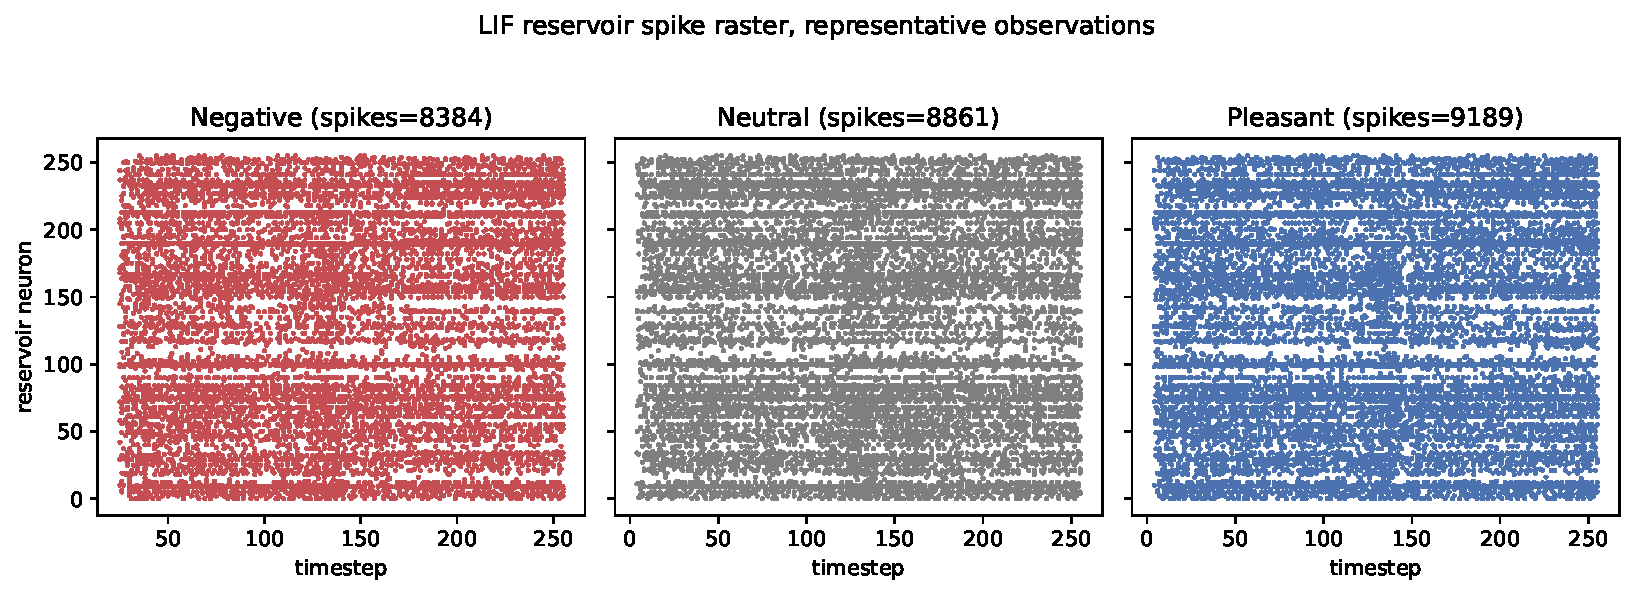
\includegraphics[width=3.6cm]{obs04_reservoir_spike_raster}};
\node[title, above=1.5pt of res] {Neuromorphic transformation};
\node[sub, below=1.5pt of res, text width=3.9cm] {fixed LIF spiking reservoir\\$+$ BSC$_6$ event-driven spike code};

% ---- Stage 3: four operationally distinct evidence streams ----
\node[stream, right=1.15cm of res, yshift=1.18cm] (E) {$E$~~spike embedding};
\node[stream, below=0.17cm of E] (D) {$D$~~reservoir dynamics};
\node[stream, below=0.17cm of D] (T) {$T$~~tPLV graph topology};
\node[stream, below=0.17cm of T] (C) {$C$~~structure--function coupling~$\kappa$};
\begin{scope}[on background layer]
  \node[draw, dashed, rounded corners, fit=(E)(C), inner sep=5pt] (streams) {};
\end{scope}
\node[title, above=2pt of streams.north, text width=3.6cm]
  {Four operationally distinct\\evidence streams};

% ---- Stage 4: characterization ----
\node[analysis, right=1.2cm of E, yshift=-0.10cm] (abl)
  {Mechanism ablation $+$ negative controls};
\node[analysis, below=0.19cm of abl] (per)
  {Perturbation robustness (temporal / amplitude / channel / graph)};
\node[analysis, below=0.19cm of per] (cl)
  {Closed-loop evidence accumulation (Dirichlet belief, EFE controller; offline, recorded observations)};
\begin{scope}[on background layer]
  \node[draw, dashed, rounded corners, fit=(abl)(cl), inner sep=5pt] (anal) {};
\end{scope}
\node[title, above=2pt of anal.north] {Characterization};

% ---- flow arrows ----
\draw[flow] (erp) -- (res);
\draw[flow] (res.east) -- (streams.west);
\draw[flow] (streams.east) -- (anal.west);

\end{tikzpicture}
\end{document}
